\documentclass[preprint]{acm_proc_article-sp}
%\documentclass[preprint]{sig-alternate}
\usepackage{url}
\usepackage{graphicx,subfigure}
\usepackage{xspace}

\newcommand{\ie}{{\em i.e.,}~}
\newcommand{\eg}{{\em e.g.,}~}
\newcommand{\HadoopBM}{HadoopBinMem\xspace}

\newenvironment{denseitemize}{
\begin{itemize}[topsep=2pt, partopsep=0pt, leftmargin=1.5em]
  \setlength{\itemsep}{4pt}
  \setlength{\parskip}{0pt}
  \setlength{\parsep}{0pt}
}{\end{itemize}}

\newcommand{\eat}[1]{}

\begin{document}

\title{Shark: Devouring Big Data}

\numberofauthors{5}
\author{
Cliff Engle,
Antonio Lupher,
Reynold Xin\\\\
UC Berkeley CS294-42 Project Report\\
\texttt{\{cengle, alupher, rxin\}@cs.berkeley.edu}
}

\maketitle
\begin{abstract}
Shark is a research data analysis system built on a novel coarse-grained distributed shared-memory abstraction. Shark marries query processing with deep data analysis, providing a unified system for easy data manipulation using SQL and pushing sophisticated analysis closer to data. It scales to thousands of nodes in a fault-tolerant manner. Shark can answer queries 40X faster than Apache Hive and run machine learning programs 25X faster than MapReduce programs in Apache Hadoop on large datasets.
\end{abstract}

% A category with the (minimum) three required fields
\category{H.2}{Database Management}{Systems}

\terms{DESIGN, MANAGEMENT}

\keywords{Databases, Data Warehouse, Machine Learning}


%%%%%%%%%%%%%%%%%%%%%%%%%%%%%%%%%%%%%%%%%%%%%%%%%%%%%%%%%%%%%%%%%%%%%%%%%%%%%%%
%%%%%%%%%%%%%%%%%%%%%%%%%%%%%%%%%%%%%%%%%%%%%%%%%%%%%%%%%%%%%%%%%%%%%%%%%%%%%%%
%%%%%%%%%%%%%%%%%%%%%%%%%%%%%%%%%%%%%%%%%%%%%%%%%%%%%%%%%%%%%%%%%%%%%%%%%%%%%%%


\section{Introduction}

Modern data analysis employs statistical methods that go well beyond the roll-up and drill-down capabilities provided by traditional enterprise data warehouse (EDW) solutions. Data scientists appreciate the ability to use SQL for simple data manipulation but rely on other systems for machine learning on these data. What is needed is a system that consolidates both. For sophisticated data analysis at scale, it is important to exploit in-memory computation.  This is particularly true with machine learning algorithms that are iterative in nature and exhibit strong temporal locality. Main-memory database systems use a \emph{fine-grained} memory abstraction in which records can be updated individually. This fine-grained approach is difficult to scale for massive datasets to hundreds or thousands of nodes in a fault-tolerant manner. In contrast, a \emph{coarse-grained abstraction}, in which transformations are performed on an entire collection of data, has been shown to scale more easily
\footnote{MapReduce is an example of coarse-grained updates as the same map and reduce functions are executed on all records.}.

\subsection{Coarse-grained Distributed Memory}
We have previously proposed a new distributed memory abstraction for in-memory computations on large clusters called Resilient Distributed Datasets (RDDs) \cite{spark-tr}. RDDs provide a restricted form of shared memory, based on coarse-grained transformations on immutable collections of records rather than fine-grained updates to shared states. RDDs can be made fault-tolerant based on lineage information rather than replication. When the workload exhibits temporal locality, programs written using RDDs outperform systems such as MapReduce by orders of magnitude. Surprisingly, although restrictive, RDDs have been shown to be expressive enough to capture a wide class of computations, ranging from more general models like MapReduce to more specialized models such as Pregel.

It might seem counterintuitive to expect memory-based solutions to help when petabyte-scale data warehouses prevail. However, it is unlikely, for example, that an entire EDW fact table is needed to answer most queries. Queries usually focus on a particular subset or time window, \eg http logs from last month, touching only the (small) dimension tables and a small portion of the fact table. Thus, in many cases it is plausible to fit the working set into a cluster's memory. In fact, \cite{memento-hotos} analyzed the access patterns in the Hive warehouses at Facebook and discovered that for the vast majority (96\%) of jobs, the entire inputs could fit into a fraction of the cluster's total memory.

\subsection{Introducing Shark}
The goal of the Shark (Hive on Spark) project is to design a data warehouse system capable of deep data analysis using the RDD memory abstraction. It unifies the SQL query processing engine with analytical algorithms based on this common abstraction, allowing the two to run in the same set of workers and share intermediate data.

Apart from the ability to run deep analysis, Shark is much more flexible and scalable compared with EDW solutions. Data need not be extracted, transformed, and loaded into the rigid relational form before analysis. Since RDDs are designed to scale horizontally, it is easy to add or remove nodes to accommodate more data or faster query processing. The system scales out to thousands of nodes in a fault-tolerant manner. It can recover from node failures gracefully without terminating running queries and machine learning functions.

Compared with disk-oriented warehouse solutions and batch infrastructures such as Apache Hive \cite{hive}, Shark excels at ad-hoc, exploratory queries by exploiting inter-query temporal locality and also leverages the intra-query locality inherent in iterative machine learning algorithms. By efficiently exploiting a cluster's memory using RDDs, queries previously taking minutes or hours to run can now return in seconds. This significant reduction in time is achieved by caching the working set of data in a cluster's memory, eliminating the need to repeatedly read from and write to disk.

In the remainder of this project report, we sketch Shark's system design and give a brief overview of the system's performance. Due to space constraints, we refer readers to \cite{spark-tr} for more details on RDDs.



\section{Apache Hive}

Hive is an open-source data warehouse system built on top of Hadoop. It supports queries in a  SQL-like declarative query language, which is compiled into a directed acyclic graph of MapReduce jobs to be executed on Hadoop. Like traditional databases, Hive stores data in tables consisting of rows, where each row consists of a specified number of columns. The query language, HiveQL is a subset of SQL that includes certain extensions, including multitable inserts, but lacks support for transactions, materialized views and has limited subquery support. 

Figure \ref{fig:hivearch} shows an overview of the architecture of Hive. A number of external interfaces are available including command line, web UI, Thrift, JDBC, and ODBC interfaces. The metastore is essentially analogous to a system catalog in an RDBMS and contains a database (often MySQL or Derby) with a namespace for tables, table metadata, and partition information. Table data is stored in an HDFS directory, while a partition of a table is stored in a subdirectory within that directory. Buckets can cluster data by column and are stored in a file within the leaf level directory of a table or partition. Hive allows data to be included in a table or partition without having to transform it into a standard format, saving time and space for large data sets. This is achieved with support for custom SerDe (serialization/deserialization) java interface implementations with corresponding object inspectors. 

\begin{figure}[t]
	\centering
	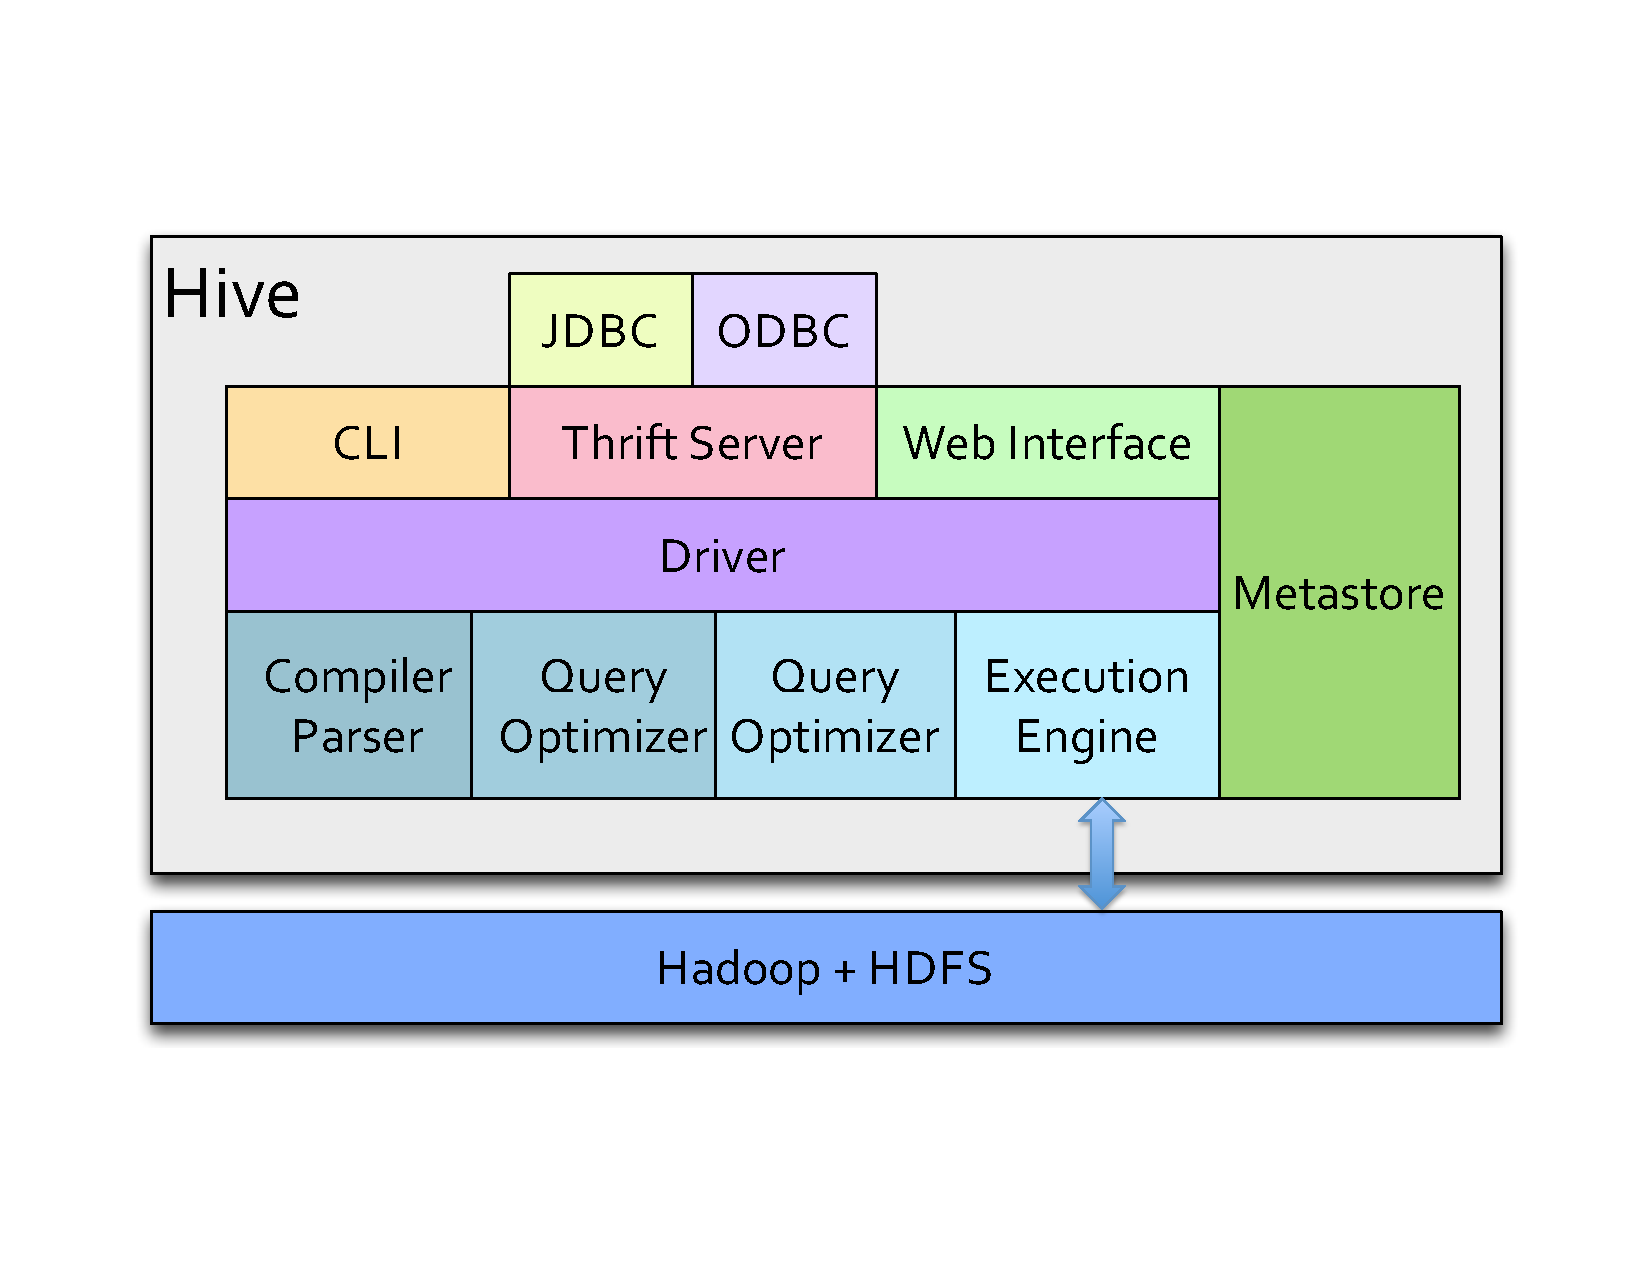
\includegraphics[width=\linewidth]{files/architecture-hive.pdf}
	\caption{Hive Architecture}
	\label{fig:hivearch}
\end{figure}


The Hive driver controls the processing of queries, coordinating their compilation, optimization, and execution. On receiving a HiveQL statement, the driver invokes the query compiler, which generates a directed acyclic graph (DAG) of map-reduce jobs for inserts and queries, metadata operations for DDL statements, or HDFS operations for loading data into tables. The Hive execution engine then executes the tasks generated by the compiler and interacts directly with Hadoop.

The generation of a query plan DAG shares many steps with a traditional database. A parser first turns a query into an abstract syntax tree (AST). The semantic analyzer turns the AST into an internal query representation and does type-checking and verifies column names. The logical plan generator then creates a logical plan as a tree of logical operators from the internal query representation. The optimizer rewrites the logical plan to add predicate pushdowns, early column pruning, repartition operators to mark boundaries between map and reduce phases, and to combine multiple joins on the same join key. The physical plan generator transforms the logical plan into a physical plan DAG of MapReduce jobs.



\section{Resilient Distributed Datasets (RDDs)}

A Resilient Distributed Dataset (RDD) is an immutable partitioned collection of records. An RDD can only be created through deterministic operations called \emph{transformations} on either data in stable storage or other RDDs. Examples of transformations include map, filter, and join.

RDDs do not need to be materialized at all times. Instead, each RDD contains lineage information about how it was derived from other datasets to compute its partitions from data in stable storage. This provides fault tolerance, since any RDD can be reconstructed after a failure using the lineage information. 

Users can also control the persistence and partitioning of RDDs. Users can indicate which RDDs they will reuse and choose a storage strategy for them (e.g., keeping them in memory). They can also ask that an RDD's elements be partitioned across machines based on key in each record. This is useful for placement optimizations, such as ensuring that two datasets that will be joined together are hash-partitioned in the same way.

Spark is a Scala implementation that exposes RDDs through a language-integrated API, where each dataset is represented as an object and transformations are invoked using methods on these objects. RDDs can either be defined through transformations (\eg map, filter) on data in stable storage or on other RDDs. Programmers can then use these RDDs in operations that return a value to the application or export data to stable storage. These operations, which cause the RDD to be 'computed' or materialized, are called \emph{actions} and include reduce, count, collect, and save. 

While each individual RDD itself is immutable, a mutable state abstraction can still be simulated with RDDs. A chain of RDDs can represent different versions of a dataset, with the transformations used to create each RDD analogous to changes made to mutable state. RDDs are evaluated lazily, allowing for pipelined transformations. Spark allows programmers to specify whether an RDD should be persistent and keeps persistent RDDs in memory by default, although the data can be spilled to disk if there is insufficient memory. Users can also specify persistence priorities for RDDs to control which collections are spilled to disk first.

\section{System Overview}

For ease of adoption, we have designed Shark to be entirely hot-swappable with Hive. Users can run Shark in an existing Hive warehouse. Queries will return the same set of results in Shark, albeit much faster in most cases, without any modification to the data or queries themselves.

We have implemented Shark using Spark, a system that provides the RDD abstraction through a language-integrated API in Scala, a statically typed functional programming language for the Java VM. Each RDD dataset is represented as a Scala object, while the transformations are invoked using methods on those objects. 

A Shark cluster consists of masters and workers. A master's lifetime can span one or several queries. The workers are long-lived processes that can store dataset partitions and intermediate RDDs resulting from transformations in memory across operations. When the user runs a query, the client connects to a master, which defines RDDs for the workers and invoke operations on them. %[Mention Mesos here?]

Figure \ref{fig:arch} shows the general architecture of Shark. Data is stored physically in the underlying distributed file system HDFS. Shark uses the Hive metastore without modification to track table metadata and statistics, much like the system catalog found in traditional RDBMS. The Shark CLI driver replaces the Hive CLI and invokes the Shark runtime driver. The Shark runtime uses Hive's functionality for parsing and compilation of HiveQL queries into a query plan. This query plan is then passed to Shark operators, which use Spark, which is loaded as a library, to create and transform RDD representations of the table data. Caching is done at the operator level by serializing query plan operator subtrees and enabling persistence on RDDs.

\begin{figure}[t]
	\centering
	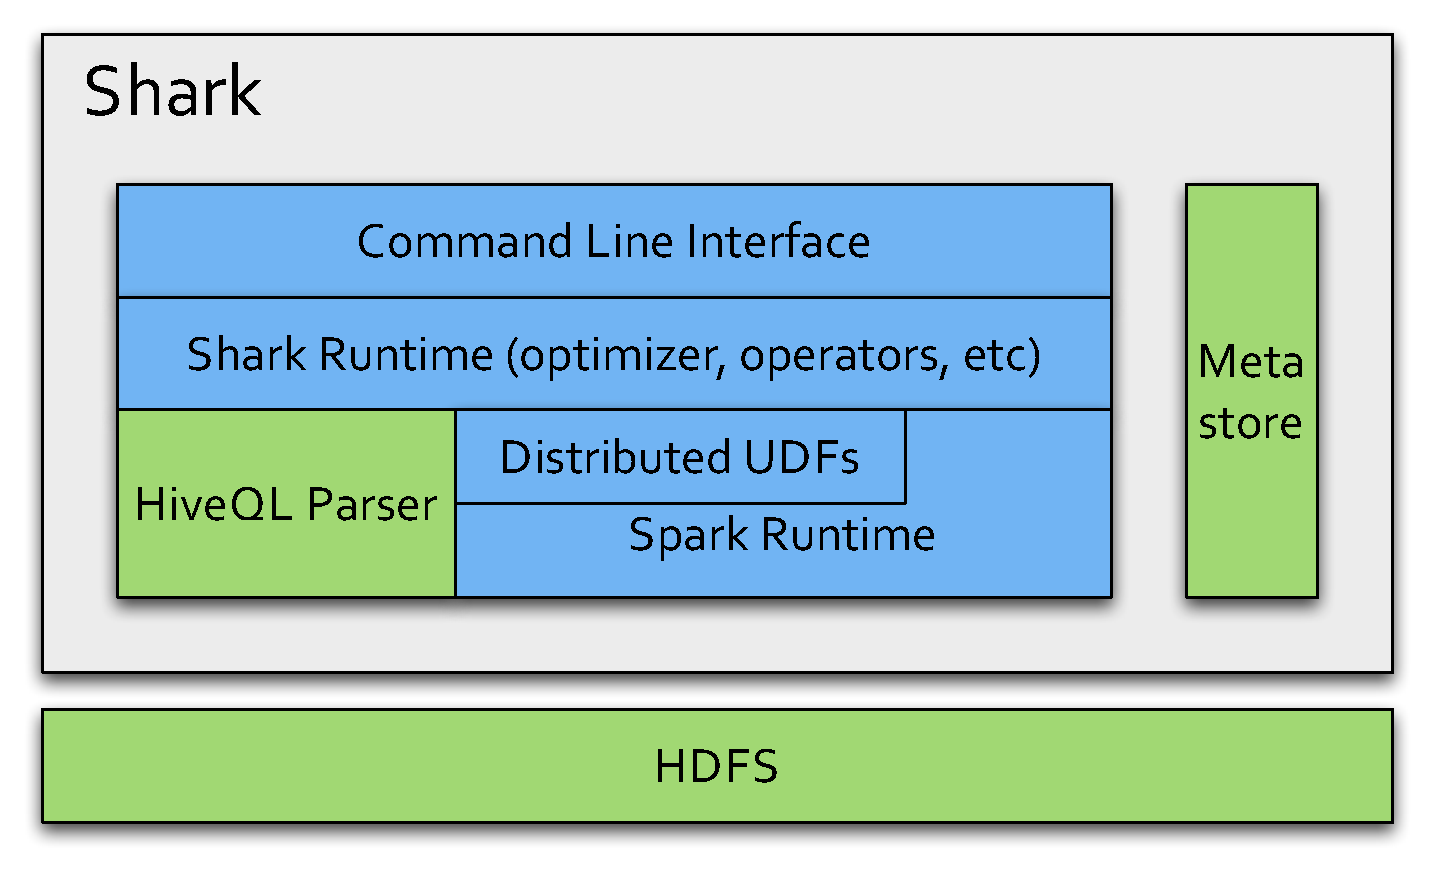
\includegraphics[width=\linewidth]{files/architecture.pdf}
	\caption{Shark Architecture}
	\label{fig:arch}
\end{figure}


\section{Query Processing}

\subsection{Overview}

At a higher level, Shark's query execution consists of three steps similar to those of a traditional RDBMS: query parsing, logical plan generation, and physical plan generation. Hive provides a SQL-like declarative query language, HiveQL, which supports standard operators including select, project, join, aggregate, union, and from clauses with sub-queries. HiveQL statements are compiled into lower level operators, which, in Hive, are executed as a sequence of MapReduce programs. Shark uses Hive as a third-party Java library for query parsing and logical plan generation. The main difference is in the physical plan execution, as Shark has its own operators written specifically to exploit the benefits provided by RDDs.

Given a HiveQL query, the Hive query compiler parses the query and generates an abstract syntax tree. The tree is then turned into the logical plan and basic logical optimization such as predicate pushdown is applied. Shark uses the existing Hive code for each of these steps. In Hive, this operator tree would then be converted into a physical plan that consisted of subtrees for separate map and reduce tasks. 

In Shark, the operator tree is executed with operators that perform transformations on RDDs. An iterator traverses the operator tree and produces an immutable RDD for each operator on the tree. The initial RDD for any query over a table is created by the table scan operator and consists of a collection of the rows in the table. Subsequent operators create new RDDs by applying map, filter, join, and other transformations. Unlike Hive, which applies its operators to tables one row at a time and writes intermediate data between MapReduce jobs to disk, in Shark, an RDD produced by an operator is not materialized until the execution engine returns the query results. At this time, the contents of the final RDD are computed by applying the appropriate transformations to the RDDs of previous operators.

Much of the common structure of Hive operators is retained in order to ensure interoperability with HiveQL. Shark currently supports all of the essential Hive operators. We reuse all of Hive's data model and type system, in addition to supporting Hive's user-defined functions, user-defined aggregate functions, custom types, and custom serialization/deserialization methods.

While the transformations available in Spark were sufficient to express most Hive operators, we had to modify Spark to implement sorting on RDDs for 'order by' clauses and to implement full outer joins. 
% any other modifications to spark?

\subsection{Caching}

A major advantage of Shark over Hive lies in its inter-query caching of data. The Spark framework provides a simple mechanism to cache RDDs in memory across clusters and recompute RDDs in the event of failures. In Shark, the resulting RDD generated by each operator subtree can be cached automatically, and a signature is computed for the subtree. This signature and a reference to the associated RDD is stored in an in-memory hash table. Signatures are computed for subsequent query subtrees and are compared to those in the table and, in the case of a match, the in-memory RDD is utilized. 

Cache invalidation is handled by checking the timestamp of the last modification of the HDFS data to the timestamp stored in our table. Spark currently supports a least recently used (LRU) policy, but we are in the process of implementing least frequently used (LFU) and are exploring more sophisticated algorithms that perform cost-based analysis for intermediate data. 

Currently, Shark automatically caches all RDDs generated by operators. Users can prevent the RDDs generated by certain operators via a global configuration file. This helps avoid filling available memory with, for example, the RDDs created by table scans on large tables, when subsequent queries perform similar filtering to narrow down the result set.

%\subsection{Implementation Details}
%The Shark code base consists of approximately 2300 lines of Scala code. The Shark driver replaces the Hive 
% driver and controls query plan execution,

% reducesink and the way we avoid writing intermediate data 
% shuffles and advantages of hash joins 
% various optimizations like kryo serialization

% Maybe mention:
% � challenges, esp. those of integrating Hive with Spark;
% - serdes 
% - gc issues
%  - how we did it orginally, what happened, how we fixed it using lazy serialization
% - challenges that this presents for caching
% mention recent modifications to spark

% talk about explicit memory management in hive vs. spark and what problems this seems to pose





\section{Shark Example}

\subsection{Query Execution Example}

Consider a Twitter-like application where users can broadcast short status messages and each user has certain profile information \eg age, gender, and location. The status messages themselves are kept in a \emph{messages} table along with a unique user identifier. Due to the volume of messages, they are partitioned by date. A \emph{profiles} table contains user information including country, gender, and age for each user id. 

{\small
\begin{verbatim}
CREATE TABLE messages (user_id INT, message STRING) 
    PARTITIONED BY (ds STRING);
CREATE TABLE profiles (user_id INT, country STRING, age INT);

LOAD DATA LOCAL INPATH '/data/messages'
INTO TABLE messages PARTITION (ds='2011-12-07');
LOAD DATA LOCAL INPATH '/data/profiles' INTO TABLE profiles;
\end{verbatim}
}

Suppose we would like to generate a summary of the top ten countries whose user have added the most status messages on Dec. 7, 2011. Furthermore, we would like to sort these results by number of messages in descending order. We could execute the following query:

{\small
\begin{verbatim}
FROM (SELECT * FROM messages a 
    JOIN profiles b ON 
    (a.user_id = b.user_id and a.ds='2011-12-07')
        ) q1
SELECT q1.country, COUNT(1) c 
    GROUP BY q1.country ORDER BY c DESC LIMIT 10
\end{verbatim}
}

The query contains a single join followed by an aggregation. Figure \ref{fig:hiveqp} is the query plan generated by Hive showing its map and reduce stages. Figure \ref{fig:sharkqp} shows the query plan as it is processed by Shark. For this query, Hive generates a three-stage map and reduce query plan. Note that the intermediate results after each MapReduce stage are written to HDFS in a temporary file in the FileSink operators. Since Spark and the RDD abstraction do not constrain us to the MapReduce paradigm, Shark can avoid this extra I/O overhead by simply writing intermediate results to local disk. Shark simply creates a new RDDs for each operator, reflecting an operator's transformation on the RDD that resulted from the previous operator's transformation. Any leaf operator is a table scan that generates an RDD from an HDFS file. 

Suppose that no previous queries have been run on this data or at least none have similar operator subtrees to the current query. At each operator stage where an RDD is substantially transformed, Shark adds the resulting RDD to the cache if caching for the given operator has not been disabled in the Shark configuration file.

\begin{figure}
	\centering
	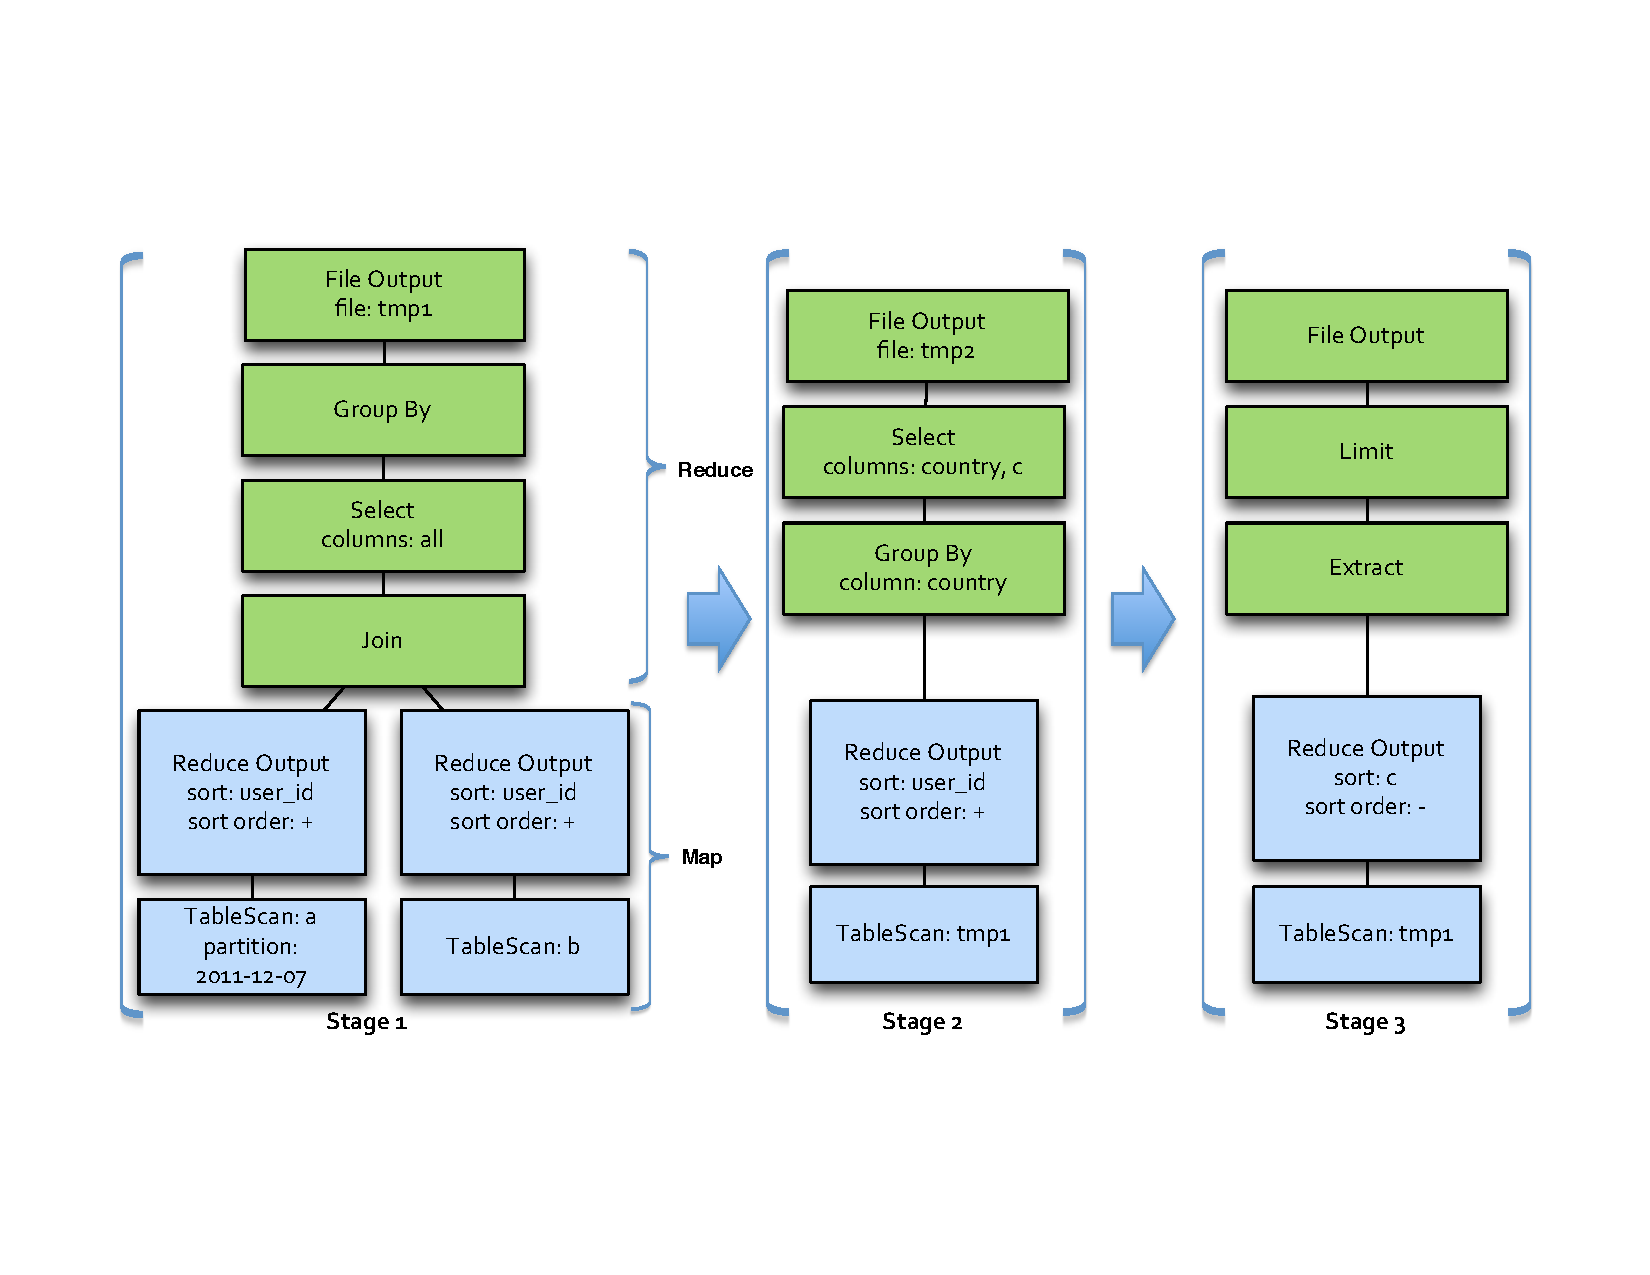
\includegraphics[width=\linewidth]{files/hive-qplan.pdf}
	\caption{Hive query plan}
	\label{fig:hiveqp}
\end{figure}

\begin{figure}
	\centering
	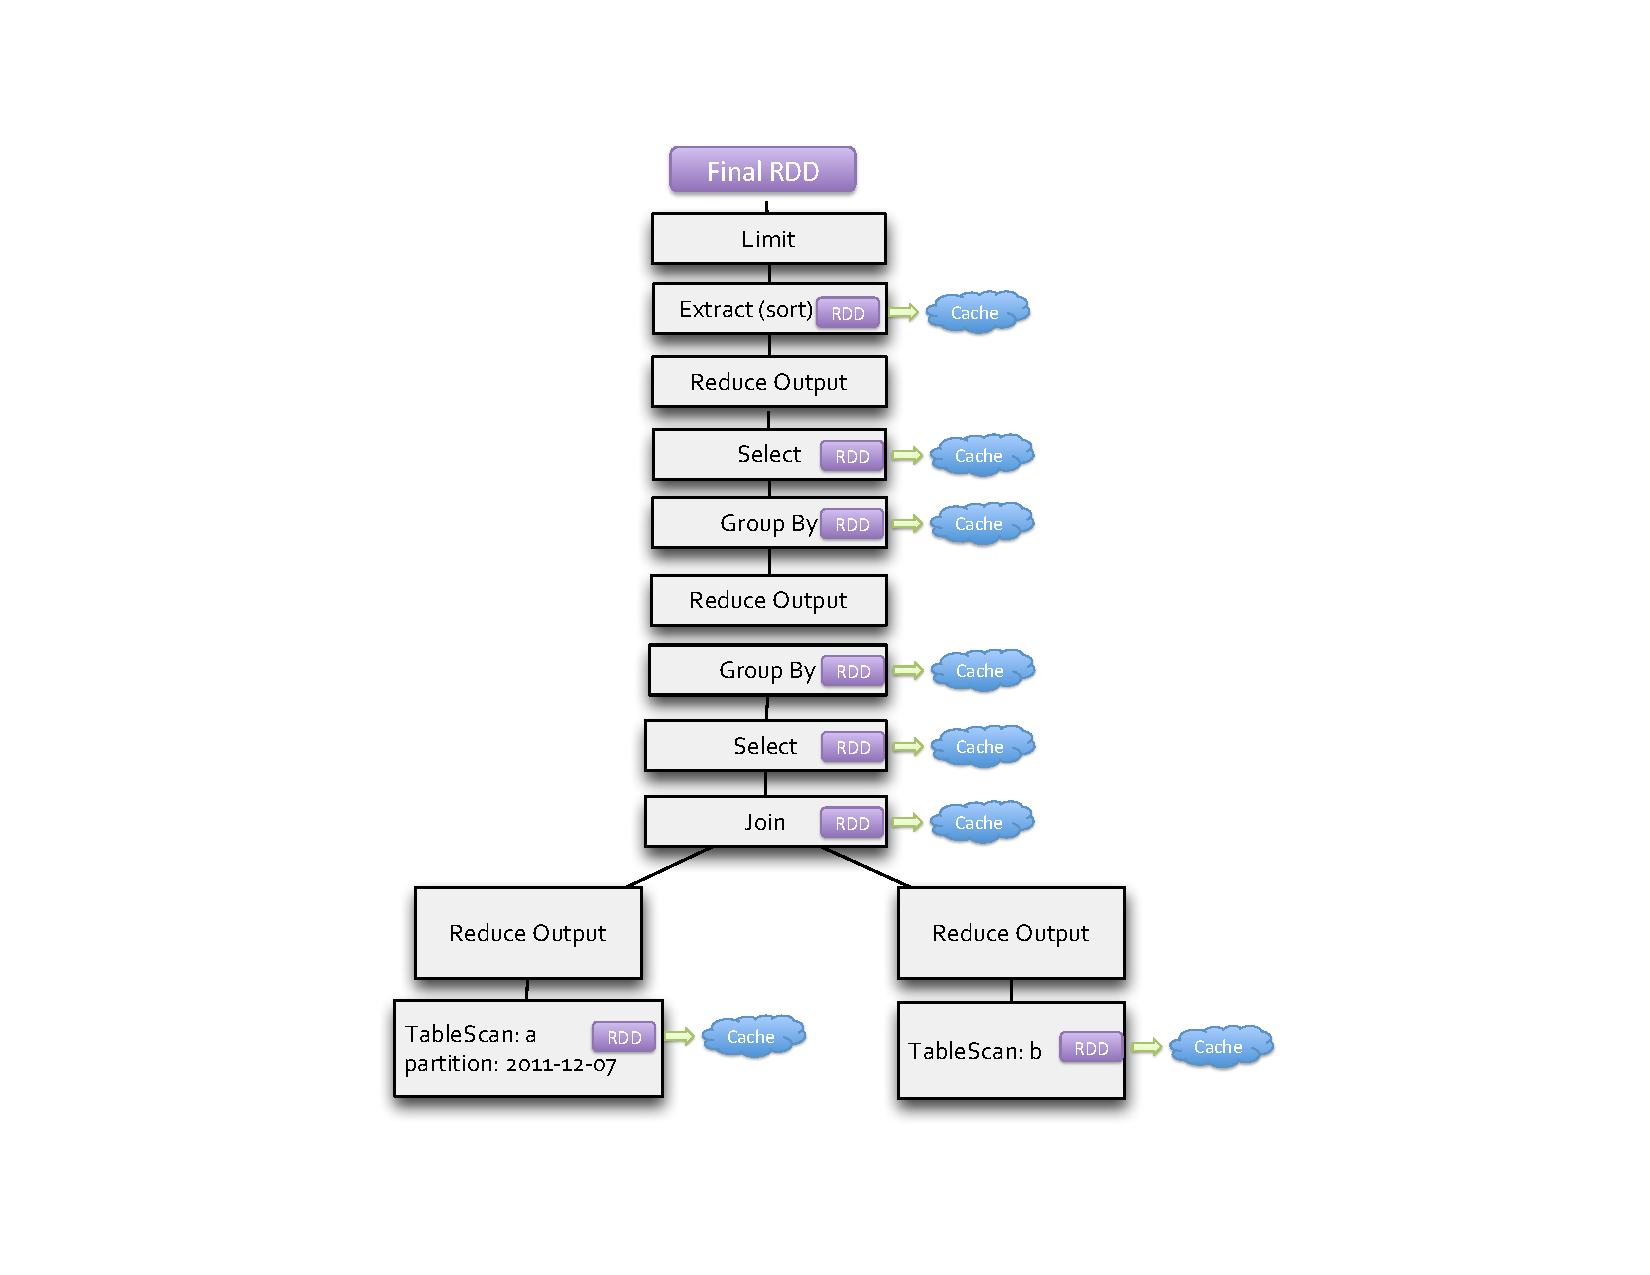
\includegraphics[width=\linewidth]{files/shark-qplan1.pdf}
	\caption{Shark query plan}
	\label{fig:sharkqp}
\end{figure}

Now, suppose that we would now like to query the same data to find the number of messages grouped by age instead. We could execute the following query. 

{\small
\begin{verbatim}
FROM (SELECT * FROM messages a 
    JOIN profiles b ON 
    (a.user_id = b.user_id and a.ds='2011-12-07')
        ) q1
SELECT q1.age, COUNT(1) c 
    GROUP BY q1.age ORDER BY age
\end{verbatim}
}

Apart from the omission of reading and writing intermediate data to HDFS, Shark's query plan is essentially identical up through the join by operator, so instead of generating new RDDs for each operation, existing RDDs for these operators will be found in memory. This is illustrated in Figure \ref{fig:sharkqp2}. The subsequent filter, group by, and order by operations require new transformations, and their resulting RDDs are stored in memory for future queries to use.

\begin{figure}
	\centering
	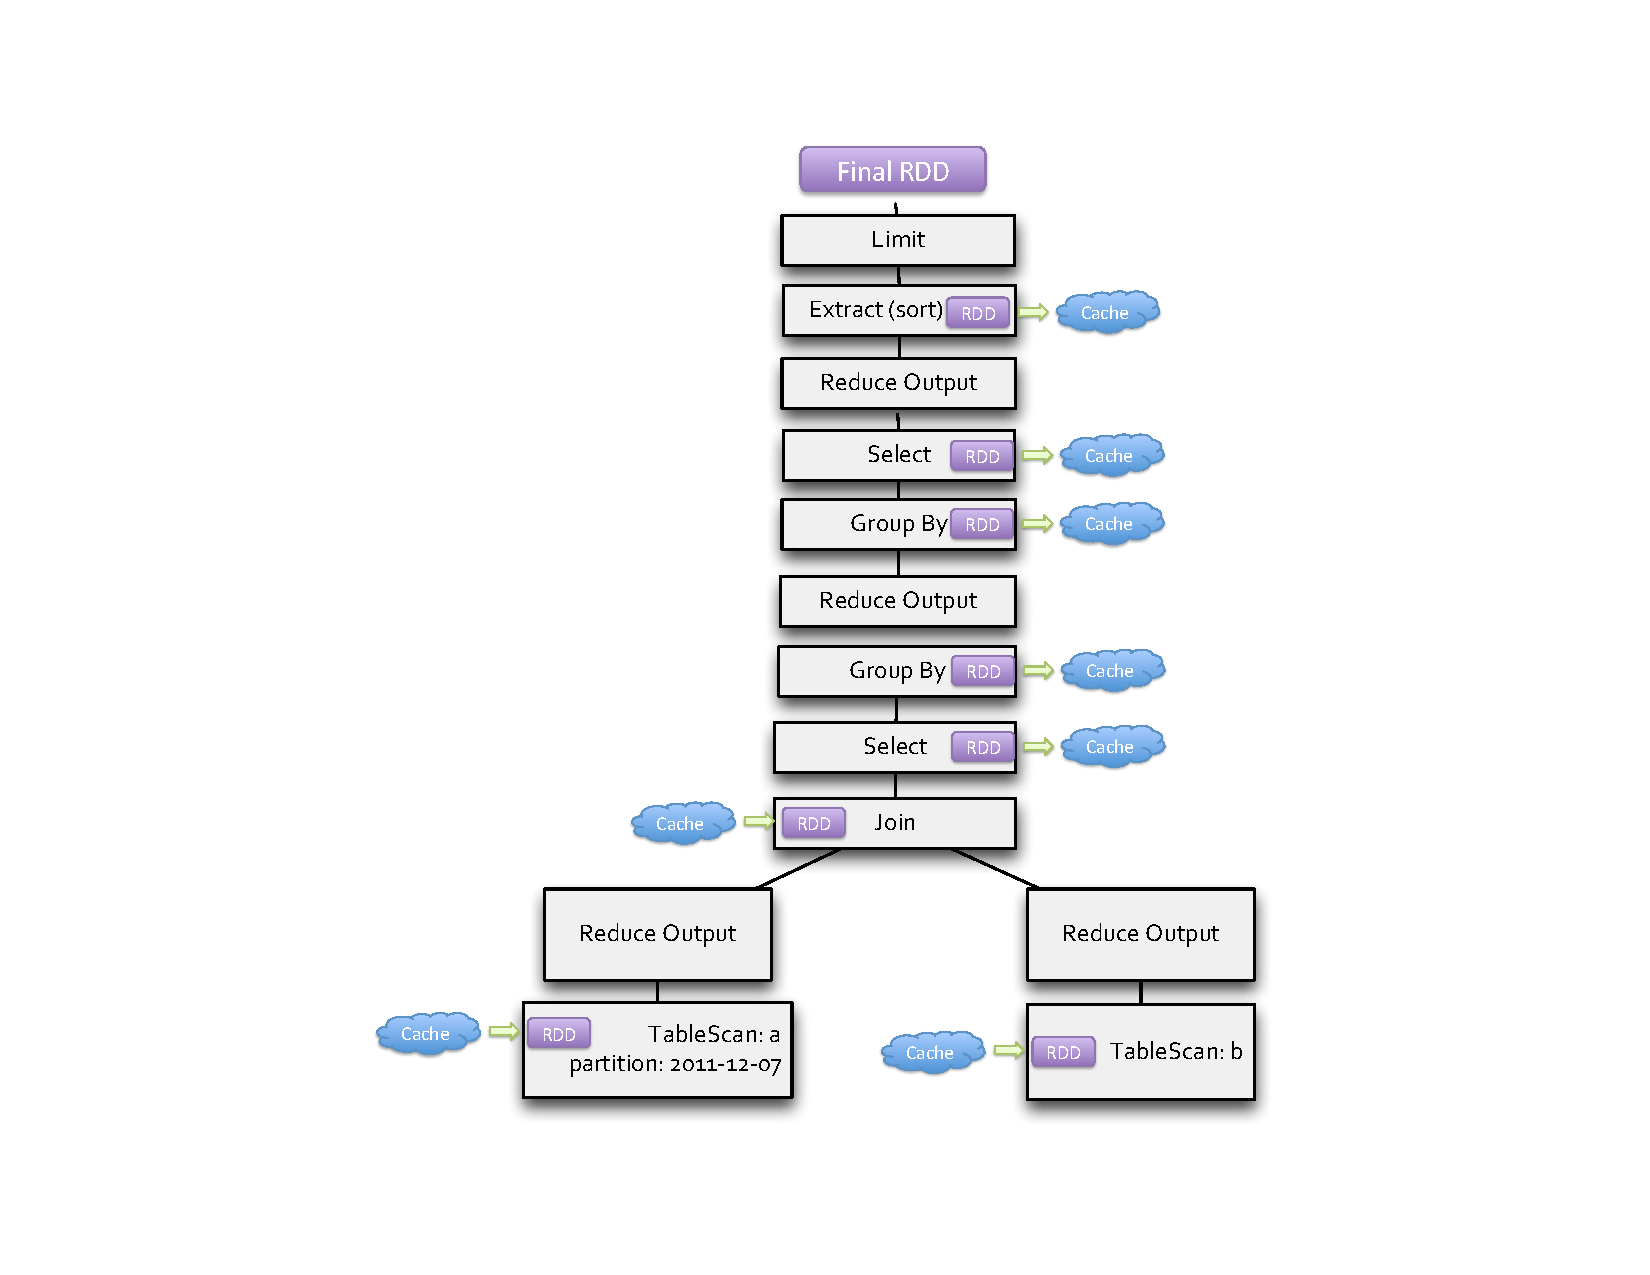
\includegraphics[width=\linewidth]{files/shark-qplan2.pdf}
	\caption{Shark query plan}
	\label{fig:sharkqp2}
\end{figure}





\section{Performance Discussions}

%We evaluated the performance of Shark and compared it with that of Hive using the TPC-H benchmark \cite{tpch} using 100GB of data on an 11-node cluster. TPC-H is the industry standard decision support benchmark, illustrating decision support systems that examine large volume of data and give answers to critical business questions.

%TPC-H is the industry standard decision support benchmark, illustrating decision support systems that examine large volume of data and give answers to critical business questions.

We evaluated the performance of Shark and compared it with that of Hive using the Brown benchmark using 72GB of data on an 11-node cluster. The benchmark was used in \cite{pavlo2009comparison} to compare the performance of Apache Hadoop versus relational database systems for large scale data processing.


\subsection{Cluster Configuration}
We used a cluster of 11 nodes on Amazon EC2 in the us-east-1b availability zone. Our experiments used High-Memory Double Extra Large Instance (m2.2xlarge) nodes with 4 cores and 34 GB of RAM. These nodes offer large memory sizes for database and memory caching applications. We used HDFS for persistent storage, with block size set to 128 MB and replication set to 3. Before each job, we cleared OS buffer caches across the cluster to measure disk read times accurately.


\subsection{Data and Queries}

\eat{
\begin{table}
	\centering
	\begin{tabular}{| l || r | r |}
		Table & File Size & Cardinality \\
		\hline
		supplier & 137M & 1M \\
		region & 389B & 5 \\
		part & 2.3G & 20M \\
		partsupp & 12G & 80M \\
		orders & 17G & 150M \\
		nation & 2.2K & 25 \\
		lineitem & 75G & 600M \\
		customer & 2.3G & 15M
	\end{tabular}
	\caption{TPC-H Table Statistics}
	\label{tb:tpch_tables}
\end{table}
}

%We used the DBGEN program provided by TPC \cite{tpch} to generate test data. Using a scaling factor of 100, we generated 100 GB of data, consisting eight tables, as documented in \ref{tb:tpch_tables}. They were first generated locally on the cluster's master node and then copied into HDFS cluster. The generation and preparation of data took approximately four hours.

%The queries we ran were adopted from \cite{tpch-hive}, which are modified from original TPC-H queries to be compatible with HiveQL while preserving the same query semantics. These queries employ varying degrees of filtering, selection, groupbys, orderbys, and aggregations.

We used the teragen and htmlgen programs \cite{pavlo2009comparison} to generate a test dataset. Using a scaling factor of 100, we generated 72 GB of data, consisting of three tables. The tables were first generated locally on the cluster's master node and then copied to the HDFS cluster. The generation and preparation of data took approximately four hours.
%, as documented in \ref{tb:tpch_tables}. 


\subsection{Performance Comparisons}

We benchmarked Shark's performance with caching enabled for the RDDs emitted by each table scan operator. We tested three different cases: while data is being cached on the first run, after the input table is cached in memory, and without any caching. Shark performs on par with or better than Hive for all of the queries in  \cite{pavlo2009comparison} on the test dataset without caching, and has more significant improvements once input data is cached. Additionally, caching data does not have a major detrimental effect on its first run. In Figure \ref{fig:query1}, we see that Shark performs equally well as Hive on un-cached data, since its runtime is dominated by loading data from disk. 

The performance improves significantly when data is cached in memory. Figure \ref{fig:query2} demonstrates that Shark has little start-up overhead, unlike Hive, which has high latency for any job. This allows Shark to provide more realtime results unlike Hive, which is realistic primarily for batch jobs. The aggregation query, Figure \ref{fig:query3}, shows similar performance on un-cached data and improvements once data is cached. The improvements due to caching are not as significant as in Query 1 or Query 2 because Shark is still limited by the shuffle phase, which requires all data to be written to disk. Finally, Figure \ref{fig:query4} shows that Shark has performance benefits for joins, primarily because Shark uses hash joins while Hive relies on Hadoop's sort-merge joins.

Since only table scan RDDs were cached in our tests, Shark's performance across first and second runs of a given query corresponds to the benefit from caching tables for queries of the same type, rather than to simply caching the final result of a query. For example, consider Query 2, which features selection and filtering. After running the query on Shark for the first time, the table data was cached in memory. Running the query for the second time benefitted from having the table data already in memory, but selection and filtering still had to be applied to the cached table data. We would expect similar performance to the second run when running a slightly different query instead, \eg selecting and filtering on different criteria. 

We would observe similar caching benefits from running the queries successively in a single Shark session. Suppose that queries 1-4 were run in succession on Shark, starting with Query 4. This query, which features a join and aggregation across the three tables would load the table data into memory, and would have an execution time of 164 seconds (1st run). Queries 3, 2, and 1 would already have their tables in memory, so their execution time would be 157, 0.7, and 6 seconds respectively (corresponding to 2nd run times), for a total of 327.7 seconds. Hive, on the other hand, would take the sum of its original execution times, or a total of 592 seconds to execute the same queries.



\begin{figure}
	\centering
	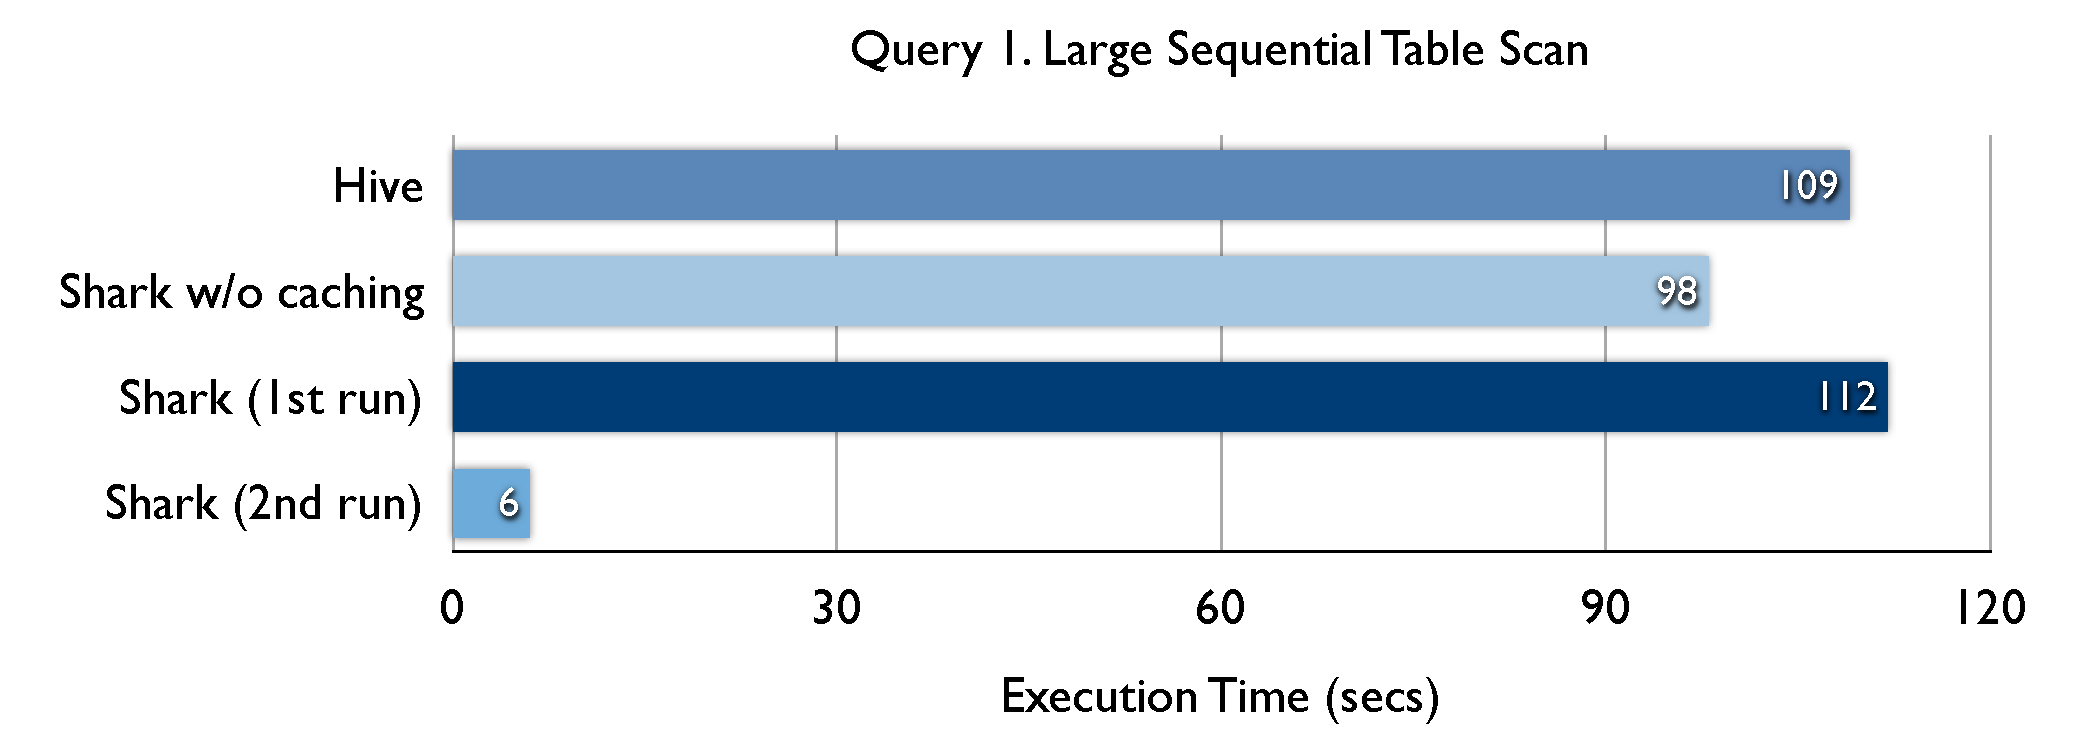
\includegraphics[width=\linewidth]{files/query1.pdf}
	\caption{Query 1 large sequential scan and grep}
	\label{fig:query1}
\end{figure}

\begin{figure}
	\centering
	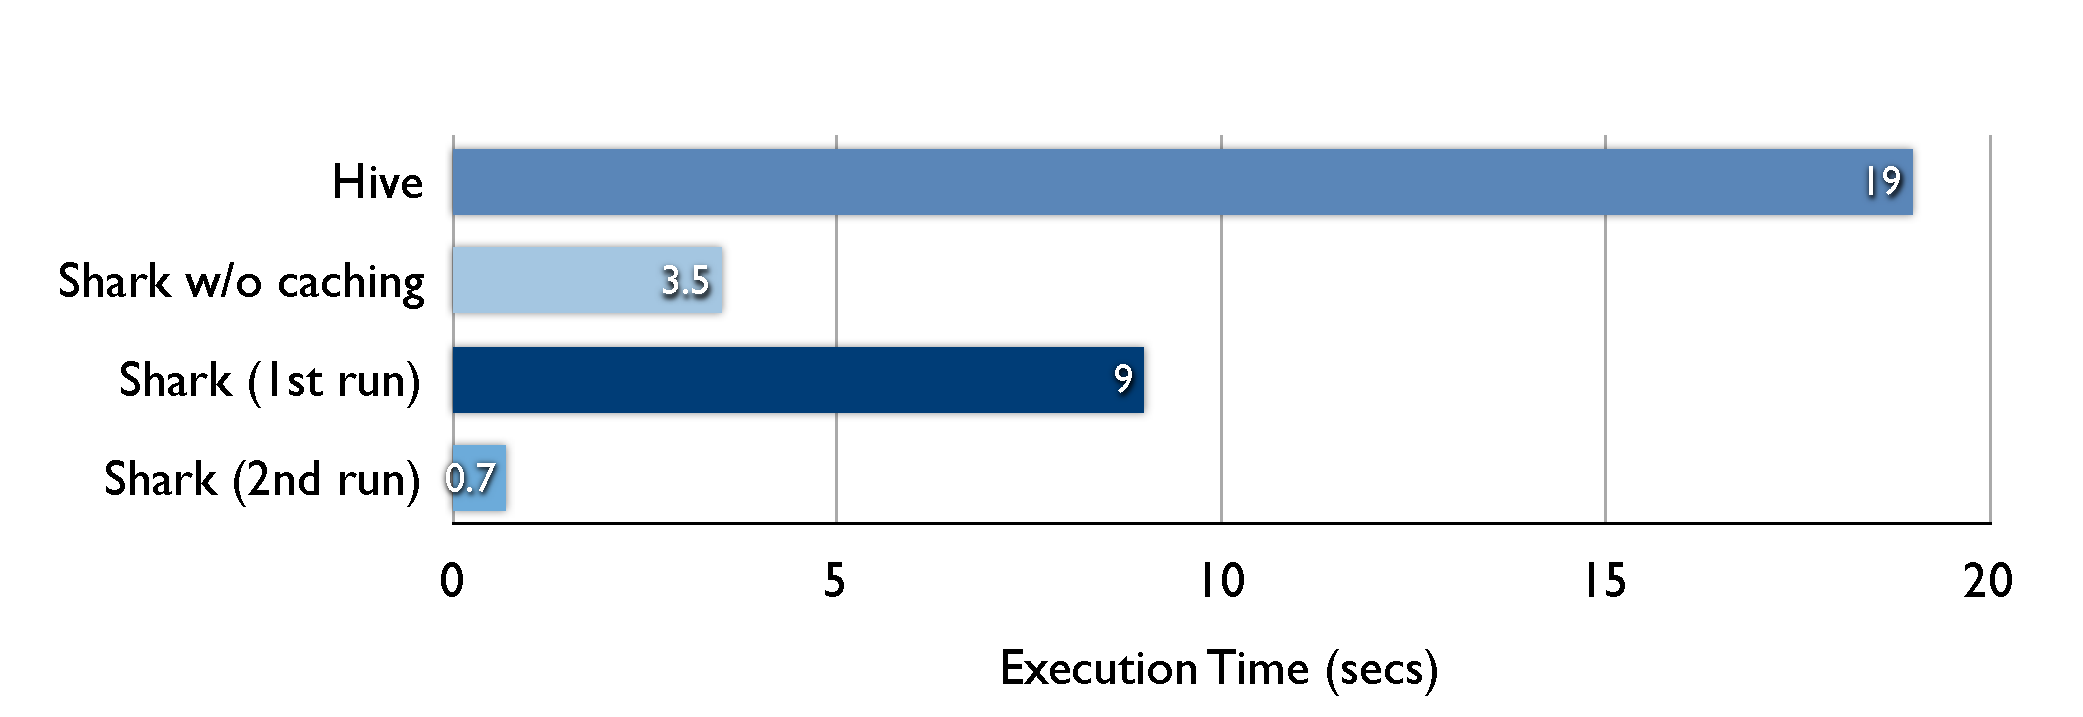
\includegraphics[width=\linewidth]{files/query2.pdf}
	\caption{Query 2 selection and filtering}
	\label{fig:query2}
\end{figure}

\begin{figure}
	\centering
	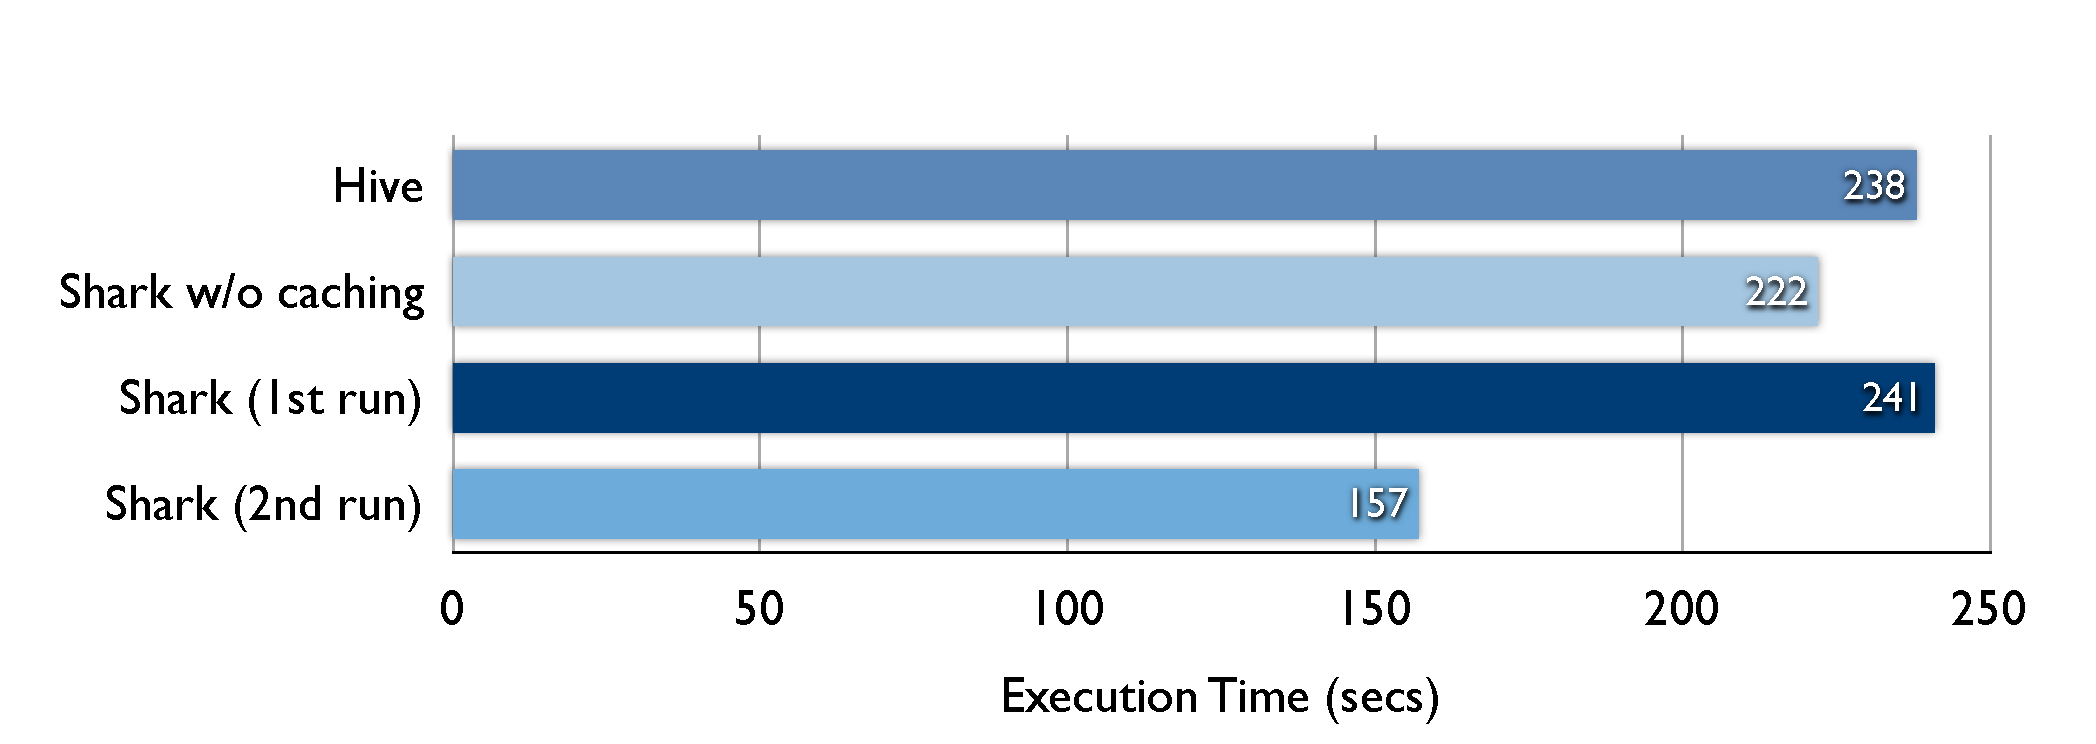
\includegraphics[width=\linewidth]{files/query3.pdf}
	\caption{Query 3 aggregation}
	\label{fig:query3}
\end{figure}

\begin{figure}
	\centering
	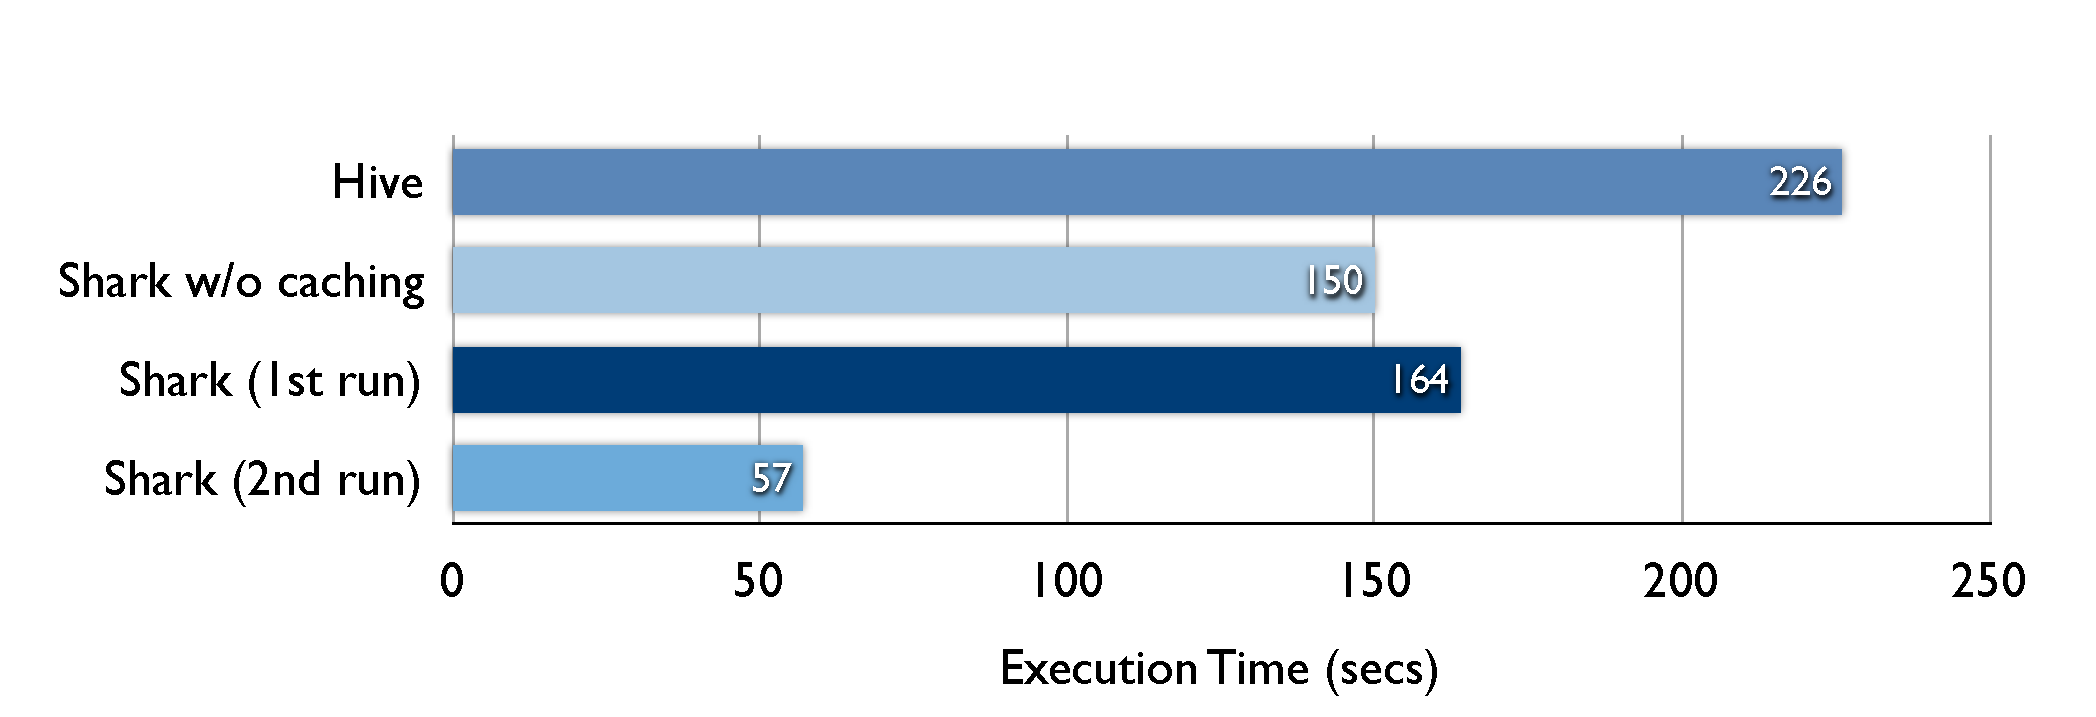
\includegraphics[width=\linewidth]{files/query4.pdf}
	\caption{Query 4 join and aggregation}
	\label{fig:query4}
\end{figure}


\subsection{JVM Memory Management}

\begin{figure}
	\centering
	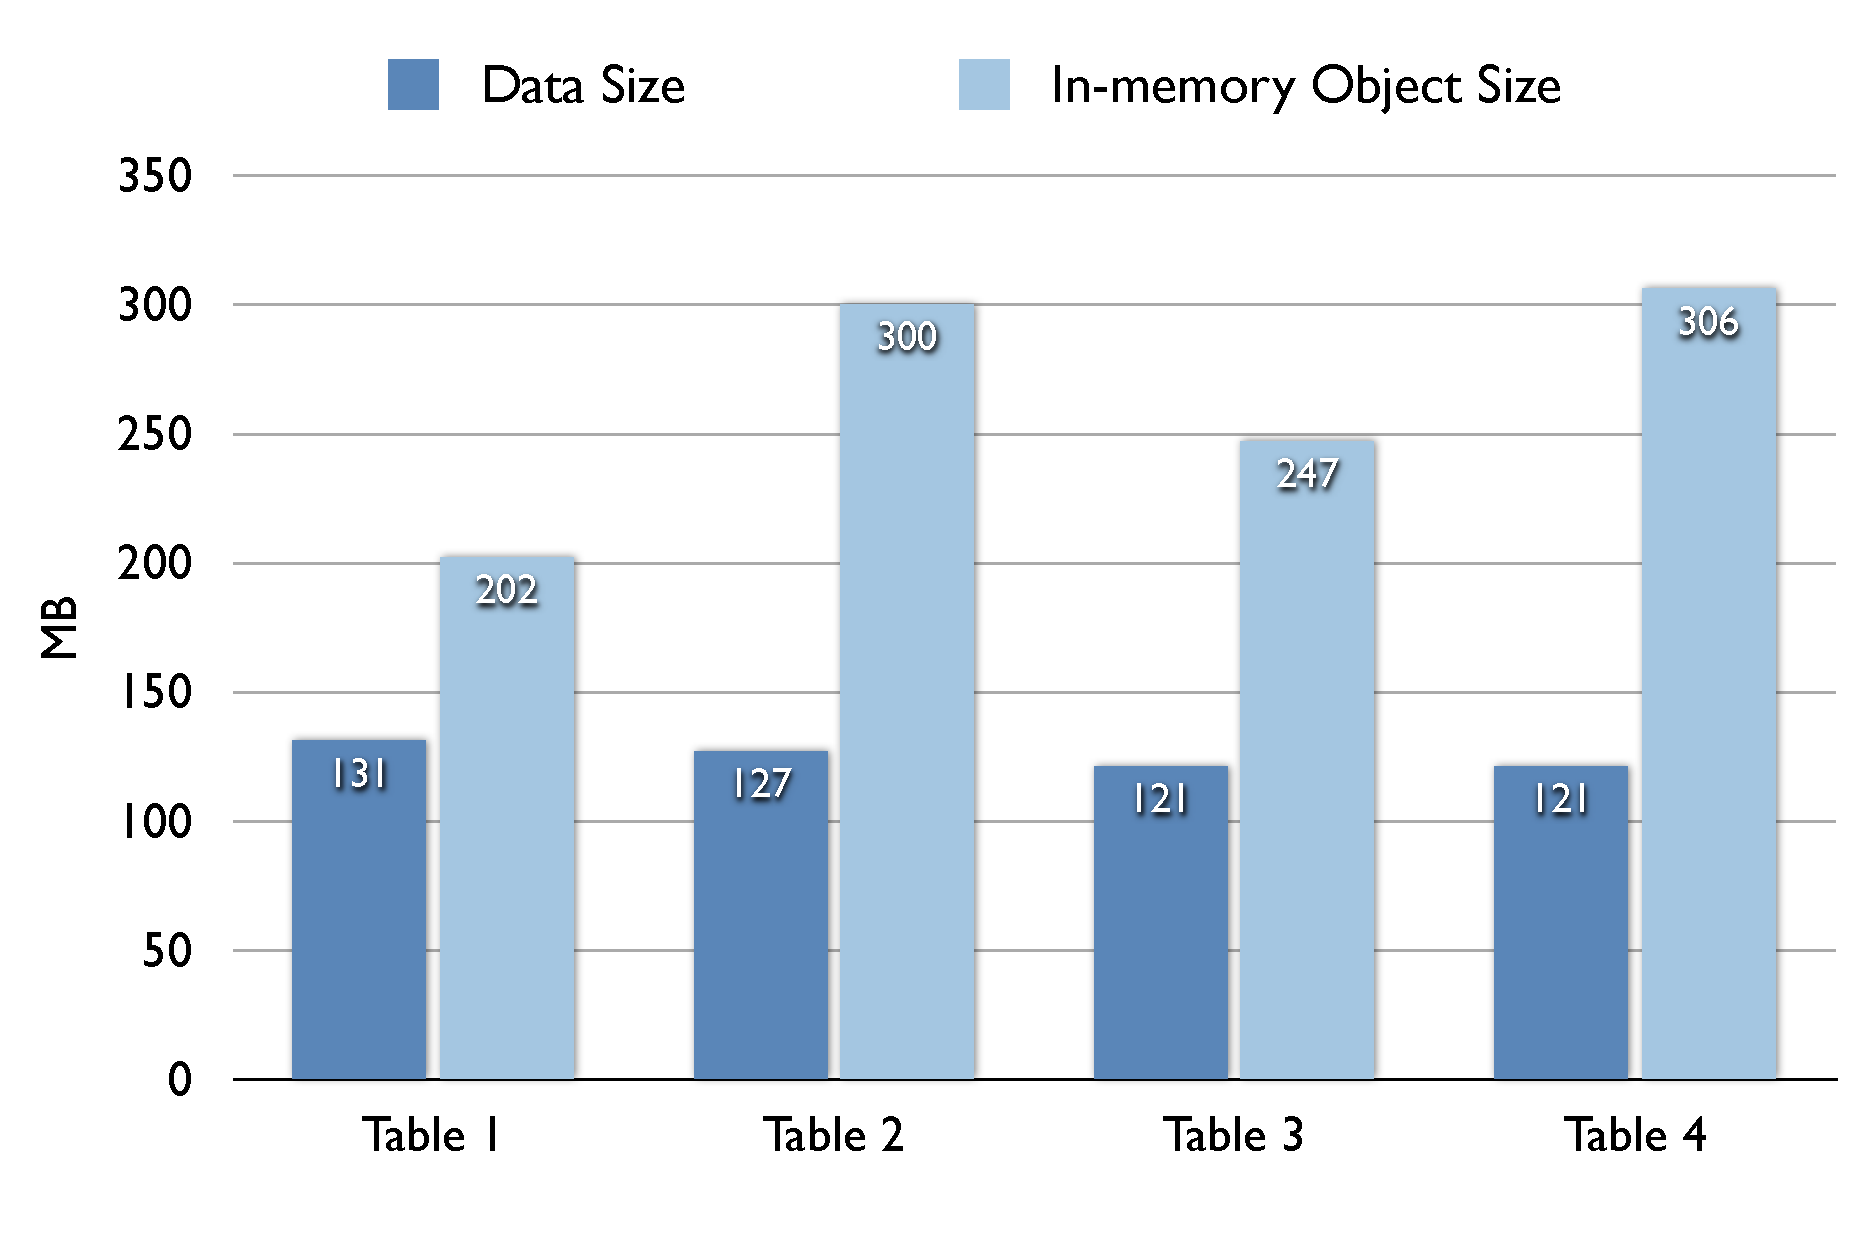
\includegraphics[width=\linewidth]{files/object-overhead.pdf}
	\caption{In-memory Java Object Overhead}
\end{figure}

Just like other programs running on top of the JVM, Shark's memory allocation and collection are managed by the JVM. There are two problems with caching large amounts of data in JVM heap. First, Cached data are considered long-lived and during their life span, they will be copied at least three times, from the eden space to the first survivor space, then to the second survivor space, and eventually to the tenured space \cite{jvm-gc}. When the long-lived data are large in size, it takes considerably large amount of time to copy the data multiple times. Second, with a very large heap, full garbage collection takes a significant chunk of time while pausing the program. Shark uses certain parts of Hive code that frequently allocates large short-lived objects. In the face of memory pressure exerted by the large data caches, these objects lead to frequent garbage collections.

The generational garbage collection is not very efficient in these cases. When we benchmarked TPC-H on Shark, with a 25GB of JVM heap space per node, normal garbage collection would take 1 - 2 seconds, while a full garbage collection would take as long as 50 seconds. When the memory usage was very high, over 90\% of the query execution time was spent in garbage collection.

This made the initial version of Shark unusable for real big data applications. We are currently studying various techniques to mitigate the problem \cite{hbase-gc}, but seem to have resolved most of these effects by implementing lazy deserialization. Our lazy deserialization dramatically improved perfomance on many of these issues by leaving deserialized rows in their original byte array format rather than converting them to Java objects. We stream the byte array through our operators and evaluate fields only when requested. Additionally, we take advantage of Spark's iterator pipelining so that we only need to keep a reference to a single byte array at a time. This allows previously used byte arrays to be garbage collected much earlier.
% add more recent performance info

%\subsection{Conviva Data Warehouse}

%Conviva Inc, a video distribution company, runs a 20 node Hive warehouse for data analytics. They have two types of queries: predefined reporting queries and ad-hoc debugging queries. 

%Their reporting queries mostly work on the same subset of the data (records matching a customer-provided predicate), but perform aggregations (averages, percentiles, and {\small\tt COUNT DISTINCT}) over different grouping fields, requiring separate MapReduce jobs. A typical reporting query takes 20 hours to run on 200 GB of compressed data. They experimented with an earlier prototype of Shark that required the developers to hand code the query plans. The query now runs in 30 mins using only two nodes with 96GB of RAM, i.e. a $40\times$ improvement in query runtime and using only 10\% of the hardware resources. The speedup comes from a combination of keeping the columns of interest in memory and avoiding repeated decompression and filtering of the same data files.

%Conviva is now running approximately 30\% of its reporting queries on the earlier prototype of Shark instead of Hive, but this requires manual porting of SQL queries. With the new version, Conviva doesn't need to rewrite their queries and will be able to achieve the same performance gains.

%In addition, a number of users at Conviva use Hive interactively for debugging \eg finding commonalities between users who experienced low video quality to identify misconfigurations and software bugs. Like the reporting queries, these queries repeatedly access and refine the same dataset, so running them over Shark would greatly reduce debug cycles.





\section{Future Work}
\label{sec:future}

Given that this was a class project, we had limited resources in our research and development. The scope of this project, however, can be extended in many dimensions and we plan to continue development after the end of the course. We separate our short-term engineering priorities from the long-term research roadmaps and document them here.

\subsection{Short-term Priorities}
There are a number of implementation details that we must tackle for Shark to be usable in real-world deployment, including:
\begin{enumerate}
    \item Better use and tuning of JVM memory management.
	\item Thrift and JDBC interfaces.
	\item In-memory materialized views: Although the long term roadmap is for the system to intelligent decide on part of the data to cache, it would be useful for users to create in-memory materialized views for fine-grained control of caching.
	\item Implement map-side join: Currently, Shark relies on the shuffle operation to join two tables, i.e. a hash-based join. This is particularly effective for joining two large tables. When one of the table is small, however, it is more efficient to ship the entire small table to all mappers, and the join operation simply becomes a filter operation on the large table. This avoids the expensive hash shuffling.
	\item Various other optimizations and Hive features including table locking, and support for multiple joins in a single shuffle phase.
	\item TPC-H data: Conduct benchmarks using 10TB TPC-H benchmark to better understand Shark's performance characteristics.
\end{enumerate}


\subsection{Long-Term Research}
As stated earlier, this is the beginning of a long term research project. We would like to explore the following topics: (1) integrated data analysis using UDFs, (2) multiple query optimization and caching, (3) in-memory columnar store, (4) in-memory compressed caching, (5) answering queries probabilistically using Quicksilver \cite{quicksilverdb}, a concurrent project developed in the AMPLab that is built on top of Shark, and (6) incremental data processing and data streaming. 

The remaining of this section is devoted to three areas of interest: efficient in-memory caching and integrated data analysis using UDFs, and multiple query optimizations.


\subsection{Efficient In-memory Caching}

At the moment, Shark RDDs cache the in-memory representation of data as Java objects. Java objects, however, have significant overheads (e.g. a 32 bit Integer object occupies 12 bytes, a 200\% overhead). Such overheads reduce the effectiveness of caching because the amount of data Shark can cache is limited. 

One way to mitigate the problem is to store RDDs in memory in columnar format. This provides benefits in two dimensions. First, Shark can store an entire column of primitive types consecutively in memory using an array, which does not involve the object overheads of Java. For tables whose columns are filled with foreign keys, this can reduce the total in-memory data structure size by up to a factor of 3. Second, columnar store enables more efficient compression \cite{cstore}. By employing computationally cheap compression algorithms on columnar structures, we expect the in-memory RDD caches will be 1/10 of what they are today.

\subsubsection{Integrated Data Analysis using UDFs}
We intend for Shark to provide a streamlined interface to unify deep data analysis with SQL query processing. It combines SQL's convenience in data manipulation with sophisticated analysis using machine learning algorithms. The analytical algorithms run in the same set of workers as the query processing engine and can reuse intermediate data in the form of RDDs created by the engine.

Shark should allow users to write UDFs in Scala to express their algorithms for distributed computation and integrate them with SQL through a special kind of table-valued user-defined functions. We plan for Shark to provide a simple API for these UDFs, which accept a \emph{Table} RDD as input and emit a \emph{Table} RDD as output. This would be implemented by wrapping the UDF interface around the Scala interpreter.

Basic machine learning algorithms, \eg linear regression, logistics regression, k-means, will be included with the Shark distribution. In most cases, the user only needs to implement a UDF that transforms the input \emph{Table} object into the desired input data type for the selected algorithm and transforms the output from the algorithm into a separate \emph{Table} object. Short UDFs can also be embedded inline in queries in Shark's interactive mode, in part thanks to the conciseness of anonymous functions in Scala.

The following example illustrates the complete process of implementing k-means clustering in Shark. The \texttt{kmeans\_core} function does the iterative k-means computation that partitions n points into k clusters represented by the centroids. \texttt{kmeans} is a UDF wrapper that converts each input record into a 2-dimensional Point object and then converts the output from \texttt{kmeans\_core} back to a Table RDD. 
{\small
\begin{verbatim}
WITH my_working_set AS (
  SELECT * FROM my_table WHERE ...
)
SELECT col1, col2, centroid FROM kmeans(my_working_set)

def kmeans(table: RDD[Table]): RDD[Table] = {
  return table.addColumn("clusterid",
    kmeans_core(table.map{
      _.get("field1"), _.get("field2") })
}

def kmeans_core(points: RDD[Point], k: Int) = {
  // Initialize the centroids.
  clusters = new HashMap[Int, Point]
  for (i <- 0 until k) centroids(i) = Point.random()

  for (i <- 1 until 10) {
    // Assign points to centroids and update centroids.
    clusters = points.groupBy(closestCentroid)
      .map{ 
         (id, points) => (id, points.sum / points.size)
      }.collectMap()
  }
}
\end{verbatim}
}

Note that since the output of the UDFs is also an RDD, the system is in closed form and the UDF output can be further processed by other Shark operators or analysis algorithms. As a syntactic sugar, users can use \texttt{\$0} to express results from the previous query.


\subsubsection{Multiple Query Optimization}
Traditional database optimizers are designed to optimize the execution of a single query. In his seminal paper on Multiple Query Optimizazation (MQO) \cite{mqo}, Sellis proposed techniques to build shared query plans from individual query plans. Krishnamurthy surveyed \cite{krishnamurthy2006shared} recent developments in MQO in his PhD dissertation. There are two types of MQO algorithms: static and dynamic. Static algorithms are easier to implement but require the system knowing the queries to be executed a priori. Dynamic algorithms are more flexible at the expense of being too sophisticated.

Static algorithms typically work very well in decision support systems such as data warehouses, where a specific set of reporting queries are predefined. Such techniques however don't work for interactive, ad-hoc data analysis. Since Shark focuses both on traditional data warehousing queries as well as ad-hoc, exploratory queries, we should investigate dynamic MQOs.





\section{Related Work}

Conceptually, Shark's operators are standard relational operators and we employ standard traditional techniques, e.g. predicate pushdowns, in distributed databases for query optimization and processing \cite{distributed-db-ozsu}. The work, however, is also inspired by a number of projects from the database community as well as the systems community.

\textbf{Massively Parallel Databases}: Since Jeff Dean et al proposed the Google MapReduce infrastructure in 2004 \cite{mapreduce} and demonstrated extreme scalability and flexibility with the system, a number of recent projects from both the industry and the academia have focused on fitting declarative data processing onto the MapReduce style computation framework. \cite{hive, pig, tenzing, hyracks, asterix} focus mostly on providing to end users a higher level declarative interface that is compiled down to MapReduce tasks. Greenplum and Aster Data have added the ability to execute MapReduce-style functions over data stored in these systems. \cite{hadoopdb, split-execution} explore on the architectural level exploiting hybrid MapReduce and relational database systems. Dremel, another project from Google \cite{dremel}, is worth mentioning as an example of a new generation of database systems that are massively distributed and run interactive queries on very large data sets. Shark differs from these projects mainly in its novel use of RDDs for caching data.

\textbf{Distributed In-Memory Computation}: A number of researchers are now focusing on in-memory solutions for cluster computing and data management. The RAMCloud project at Stanford \cite{ramcloud} aims at creating a low latency distributed hash table for a wide range of applications. RAMCloud exposes the ability to do fine-grained updates, and the entire system's write throughput is limited by the aggregated write throughput of all disks. MIT's H-Store \cite{hstore} is a distributed main memory database. It features an architecture similar to traditional relational databases, albeit optimized for memory operations. H-Store focuses mainly in transaction processing and provides ACID guarantees. In contrary, Shark is designed from ground-up to exploit RDD for data warehousing.
% maybe mention piccolo?

\textbf{Distributed Machine Learning}: One design goal of Shark is to unify data exploration in SQL and sophisticated data analyses in one system. A number of changes have been suggested to improve the standard MapReduce framework that can significantly benefit iterative machine learning jobs. For example, the HaLoop project at the University of Washington \cite{haloop} enables the specification of cyclic workflows, while the MapReduce Online project at Berkeley \cite{mapreduce-online} allows data to be piped between operators to reduce the latency of iterative jobs.

The machine learning community has been investigating what algorithms fit more naturally into this programming paradigm. \cite{MapReduceML} analyzed ten different machine learning algorithms and pointed out that 10 common machine learning algorithms belong to a family called Summation Form algorithms and can be executed in an ``embarrassingly parallel'' fashion using MapReduce. In \cite{Gillick}, Gillick proposes a taxonomy of standard machine learning algorithms: single-pass learning, iterative learning, and query-based learning with distance metrics. He then analyzes the performance characteristics of these algorithms implemented in MapReduce. Gillick also discusses the complications of using MapReduce to implement more advanced machine learning algorithms and proposes improvements, primarily shared-state among mappers and static typing, to Hadoop to ease these problems.




\section{Conclusion}

We have presented Shark, a new data analysis system that combines the coarse-grained distributed shared-memory abstraction of RDDs with the Hive data warehouse. Our working prototype provides optimized execution of ad-hoc, exploratory queries that exploit inter-query temporal locality. In contrast to Hive and other data warehouse systems, Shark takes advantage of increasing RAM capacities to keep as much intermediate data in memory as possible, fundamentally accelerating query processing for similar queries or queries over the same dataset. 
% Summarize performance results here


%\subsection{RDDs}
%RDDs provide a restricted form of shared memory, based on coarse-grained transformations on immutable collections of records rather than fine-grained updates to shared states. When the workload exhibits temporal locality, programs written using RDDs outperform by orders of magnitude programs written for other system such as MapReduce. And surprisingly, although restrictive, RDDs have been shown to be expressive enough to capture a wide class of computations, ranging from more general models like MapReduce to more specialized models such as Pregel.

%Formally, an RDD is an immutable, partitioned collection of records that can only be created through deterministic \emph{transformations} on either data in stable storage (\eg files in HDFS) or other RDDs. Examples of transformations include \emph{map}, \emph{filter}, \emph{reduce}, and \emph{join}. Note that RDDs do not need to be materialized at all times, as they can be reconstructed based on lineage information. Users can control two aspects of RDDs: \emph{persistence} and \emph{partitioning}. Using the persistence API, users can indicate which RDDs they will reuse and choose a storage strategy for them (\eg caching them in memory). This is particularly useful in cache investment as the higher level program can choose to materialize certain RDDs in memory and reuse them later. For workloads that require going through data multiple times, such as interactive queries and iterative machine learning queries, Spark's persistence feature is very attractive. They can also ask that an RDD's elements be partitioned across machines based on key in each record. This is useful for placement optimizations, such as ensuring that two datasets that will be joined together are hash-partitioned in the same way.



%Data scientists, however, appreciate using SQL to manipulate data. Traditionally, they load data into a relational database for basic analysis, and then run algorithms in external computation frameworks such as MapReduce. Shark allows the users to express deep analyses as well as simple SQL queries, and the two can effectively share the same computation resource as well as the same in-memory data.

%Although Hive was designed to be a data warehousing solution, based on our discussions with many Hive users, a large percentage of Hive queries are ad-hoc, exploratory in nature and issued from the Hive console rather than programmatically generated for traditional data warehousing reports. Take Facebook for example. Their Hadoop clusters are dominated by jobs generated from Hive \cite{hive} queries. Even though the queries are intended to be exploratory, median map and reduce job duration is 84s \cite{delay-scheduling}. Note that typical query duration would be a multiple of this number since a query consists of multiple stages of map and reduce jobs. There is a tremendous difference in interactivity between queries that run in seconds versus minutes or hours.


%%%%%%%%%%%%%%%%%%%%%%%%%%%%%%%%%%%%%%%%%%%%%%%%%%%%%%%%%%%%%%%%%%%%%%%%%%%%%%%
%%%%%%%%%%%%%%%%%%%%%%%%%%%%%%%%%%%%%%%%%%%%%%%%%%%%%%%%%%%%%%%%%%%%%%%%%%%%%%%
%%%%%%%%%%%%%%%%%%%%%%%%%%%%%%%%%%%%%%%%%%%%%%%%%%%%%%%%%%%%%%%%%%%%%%%%%%%%%%%

\section{Acknowledgments}
The authors would like to acknowledge a number of colleagues who helped develop and conduct experiments of Shark. Much thanks to Peter Alvaro, Neil Conway, Andy Konwinski, Matei Zaharia, Michael Franklin, and Ion Stoica.

This research is supported in part by gifts from Google, SAP, Amazon Web Services, Cloudera, Ericsson, General Electric, Huawei, IBM, Intel, MarkLogic, Microsoft, NEC Labs, NetApp, Oracle, Splunk, VMware and by DARPA (contract \#FA8650-11-C-7136).

\bibliographystyle{abbrv}
\bibliography{paper}

\balancecolumns
\end{document}
